\documentclass{article} % For LaTeX2e
\usepackage{iclr2017_conference,times}
\usepackage{hyperref}
\usepackage{url}
\usepackage{microtype}
\usepackage{graphicx}
\usepackage{subfigure}
\usepackage{booktabs} % for professional tables
\usepackage{amsmath, amssymb, amsthm, mathrsfs, cases, enumerate}
%\usepackage{geometry, setspace, indentfirst, subfigure, fontspec}
\usepackage{listings, xcolor, makecell, multirow, graphicx}
\usepackage{appendix}  
\usepackage{algorithm}% http://ctan.org/pkg/algorithms
\usepackage{algpseudocode}% http://ctan.org/pkg/algorithmicx
\title{Style Transfer}


\author{Guo Jiaming\\
Harvard\\
{15000@pku.edu.cn}
\And
Wang Jianqiao\\
Yuanpei College\\
{1500017822@pku.edu.cn}
}

% The \author macro works with any number of authors. There are two commands
% used to separate the names and addresses of multiple authors: \And and \AND.
%
% Using \And between authors leaves it to \LaTeX{} to determine where to break
% the lines. Using \AND forces a linebreak at that point. So, if \LaTeX{}
% puts 3 of 4 authors names on the first line, and the last on the second
% line, try using \AND instead of \And before the third author name.

\newcommand{\fix}{\marginpar{FIX}}
\newcommand{\new}{\marginpar{NEW}}

%\iclrfinalcopy % Uncomment for camera-ready version

\begin{document}
% \nipsfinalcopy is no longer used

\maketitle

\begin{abstract}
\emph{Neural Style Transfer} is a process of using \emph{Convolutional Neural Networks (CNN)} to render a content image in different styles. Our contribution includes designing and training the framework of style transfer (\cite{1508.06576}) and fast style transfer proposed by \cite{1603.08155} with pre-trained VGG Networks.
\end{abstract}

\section{Introduction}


\subsection{Very Deep Convolutional Networks (VGG)}
VGG, proposed by \cite{1409.1556}, is one of the most popular deep neural network classifiers. This network is characterized by its simplicity, using only $3×\times3$ convolutional layers stacked on top of each other in increasing depth. Reducing volume size is handled by max pooling. Two fully-connected layers, each with 4,096 nodes are then followed by a softmax classifier. Particularly, the network architecture of VGG16 and VGG19 are presented in Figure \ref{vgg} in the Appendix. Moreover, pre-trained VGG16 and VGG19 networks \footnote{Pre-trained VGG weights:\url{http://www.vlfeat.org/matconvnet/models/?C=D;O=A}} we used in this implement of style transfer were successfully trained on ImageNet.

\subsection{Style Transfer}

Transferring the style from one image onto another can be considered a problem of texture transfer, whose goal is to synthesize a texture from a source image while constraining the texture synthesis in order to preserve the semantic content of a target image. Texture transfer algorithms use only low-level image features of the target image to inform the texture transfer. Ideally, however, a style transfer algorithm should be able to extract the semantic image content from the target image and then inform a texture transfer procedure to render the semantic content of the target image in the style of the source image. Inspired by the power of \emph{Convolutional Neural Networks (CNN)}, \cite{1508.06576} proposed a framework to model the content or style of an image through a pre-trained CNN. Moreover, \emph{A Neural Algorithm of Artistic Style} was proposed to separate and recombine the image content and style of natural images, which opened up a new field--Neural Style Transfer. However, the biggest drawback of this algorithm is that it runs too slow. To tackle this, \cite{1603.08155} proposed a \emph{Fast Style Transfer} algorithm. It introduced an \emph{Image Transform Net}, a feed-forward network that is trained to solve the optimization problem proposed by \cite{1508.06576} in real-time.


\section{Model}
\label{model}
\subsection{A Neural Algorithm of Artistic Style}
\emph{A Neural Algorithm of Artistic Style}, proposed by \cite{1508.06576}, is generated on the basis of pre-trained VGG19 network, which contains 16 convolutional and 5 pooling layers. Before we introduce the algorithm (shown in Figure \ref{fig:naas}), it is of great importance to notice that what differs this style transfer framework from other deep learning networks is that the different objects they does gradient descent on. In conventional deep learning networks, the network fixes the input and trains the weights by optimizing loss function. However, in this style transfer framework, a pre-trained network is used. In other words, the network trains its input with fixed weight by optimizing its loss function.\\

The process of the algorithm is as follows: (1) let three images pass forward through pre-trained VGG19, including content image, style image, and the the initialized 'image' we want to generate. (2) optimize the loss function and revise the 'image' using a stochastic gradient descent algorithm. In the above process, the content and style images are fixed and the initialized 'image' could be a white noise or the original content (style) image. The loss function contains two parts: the content loss and the style loss.
\begin{figure}[t]
\centering
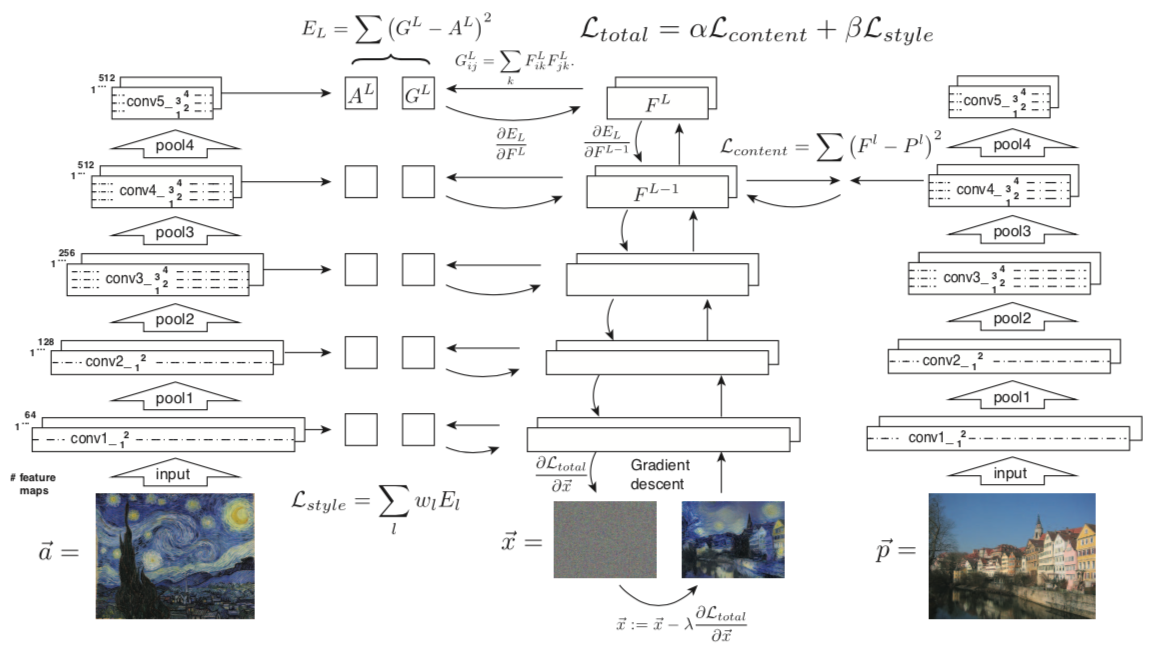
\includegraphics[scale=0.35]{neuralstyletransfer.png}
\label{fig:naas}
\caption{A Neural Algorithm of Artistic Style}
\end{figure}
\begin{itemize}
\item \textbf{Content Loss}: Let $\vec{p}$ and $\vec{x}$ be the content image and the image that is generated, and $P^l$ and $F^l\in \mathcal{R}^{N_l\times M_l}$ their respective feature representation in layer $l$, where $N_l$ and $M_l$ denotes the number of filters and the size of each feature map respectively. We then define the squared-error loss between the two feature representations as the content loss on layer $l$:
$$\mathcal{L}_{content}(\vec{p}, \vec{x}, l)=\frac{1}{2}||F^l-P^l||_F^2$$
The total content loss is  $$\mathcal{L}_{content}(\vec{p},\vec{x})=\sum_{l \text{ is a content layer}}\omega_l\mathcal{L}_{content}(\vec{p},\vec{x},l)$$ where $\omega_l$ is the weight of layer $l$.
\item \textbf{Style Loss}: Let $\vec{a}$ and $\vec{x}$ be the style image and the image that is generated, and $A^l$ and $G^l$ their respective style representation in layer $l$, which are actually the \emph{Gram matrix} of their feature representation. The contribution of layer $l$ to the total style loss is:
$$\mathcal{L}_{style}(\vec{a}, \vec{x}, l)=\frac{1}{4N_l^2M_l^2}||G^l-A^l||_F^2$$
and the total style loss is:
$$\mathcal{L}_{style}(\vec{a},\vec{x})=\sum_{l \text{ is a style layer}}\omega_{l}\mathcal{L}_{style}(\vec{a}, \vec{x}, l)$$
where $\omega_l$ is the weight of layer $l$.
\item \textbf{Total Loss}: The total loss is a combination of content loss and style loss, which is given by $$\mathcal{L}_{total}(\vec{a},\vec{p},\vec{x})=\alpha \mathcal{L}_{content}(\vec{p},\vec{x}) + \beta \mathcal{L}_{style}(\vec{a},\vec{x})$$ where $\alpha$ and $\beta$ are the weighting factors for content and style reconstruction, respectively. Moreover, the loss ration is given by $\alpha/\beta$.
\end{itemize}



\subsection{Fast Style Transfer}
\cite{1406.2661}
\cite{1603.08155}\\
\begin{figure}[h]
\centering
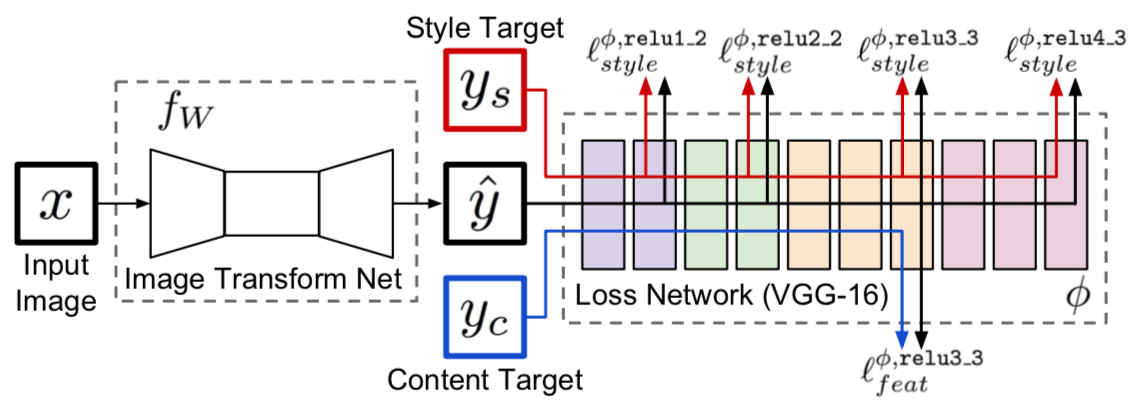
\includegraphics[scale=0.3]{fast.png}
\label{fig: fast}
\caption{Fast Style Transfer: Image Transformation Network (left) and Loss Network (right).}
\end{figure}

\begin{table}[h]
\caption{Network architecture used for style transfer networks.}
\label{transform}
\centering
\begin{tabular}{|c|c|}

\hline
\textbf{Layer}&\textbf{Activation Size}\\
\hline
Input & $3\times256\times256$\\
$32\times9\times9$ conv, stride 1 & $32\times256\times256$\\
$64\times3\times3$ conv, stride 2&$64\times128\times128$\\
$128\times3\times3$ conv, stride 2& $128\times64\times64$\\
Residual block, 128 filters&$128\times64\times64$\\
Residual block, 128 filters&$128\times64\times64$\\
Residual block, 128 filters&$128\times64\times64$\\
Residual block, 128 filters&$128\times64\times64$\\
Residual block, 128 filters&$128\times64\times64$\\
$64\times3\times3$ conv, stride 1/2&$64\times128\times128$\\
$32\times3\times3$ conv, stride 1/2&$32\times256\times256$\\
$3\times9\times9$ conv, stride 1&$3\times256\times256$\\

\hline

\end{tabular}
\end{table}


\section{Experiments}
\label{exp}





\section{Conclusion and Discussion}


\bibliography{iclr2017_conference}
\bibliographystyle{iclr2017_conference}
\newpage
\begin{appendix}
\section{VGG Networks Architecture}
\begin{figure}[ht]
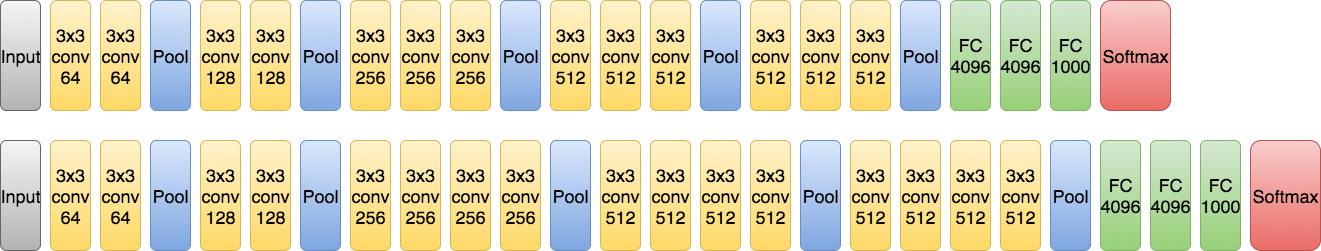
\includegraphics[scale=0.3]{VGG.png}
\caption{VGG Networks Architecture: VGG16 (above) and VGG19 (bottom).}
\label{vgg}
\end{figure}

\end{appendix}

\end{document}
